\section{High-Pass Filter}

With high values of feedback gain and depth, we can occur in the risk of saturation, in particular at low frequencies. In order to avoid that, we decided to add a high-pass filter before the wet signal line, by implementing a first-order recursive filter:
\[
	y[n] = \alpha \cdot \left( y[n-1] + x[n] - x[n-1] \right)
	\qquad
	0 \le \alpha \le 1
\]
where $\alpha$ has the same role as the time-constant of an analog RC circuit.
In particular, it is related to the cut-off frequency $f_c$ as:
\[
	\alpha = \left( \frac{2 \pi f_c}{F_s} + 1 \right)^{-1}
\]

\begin{figure}
	\centering
	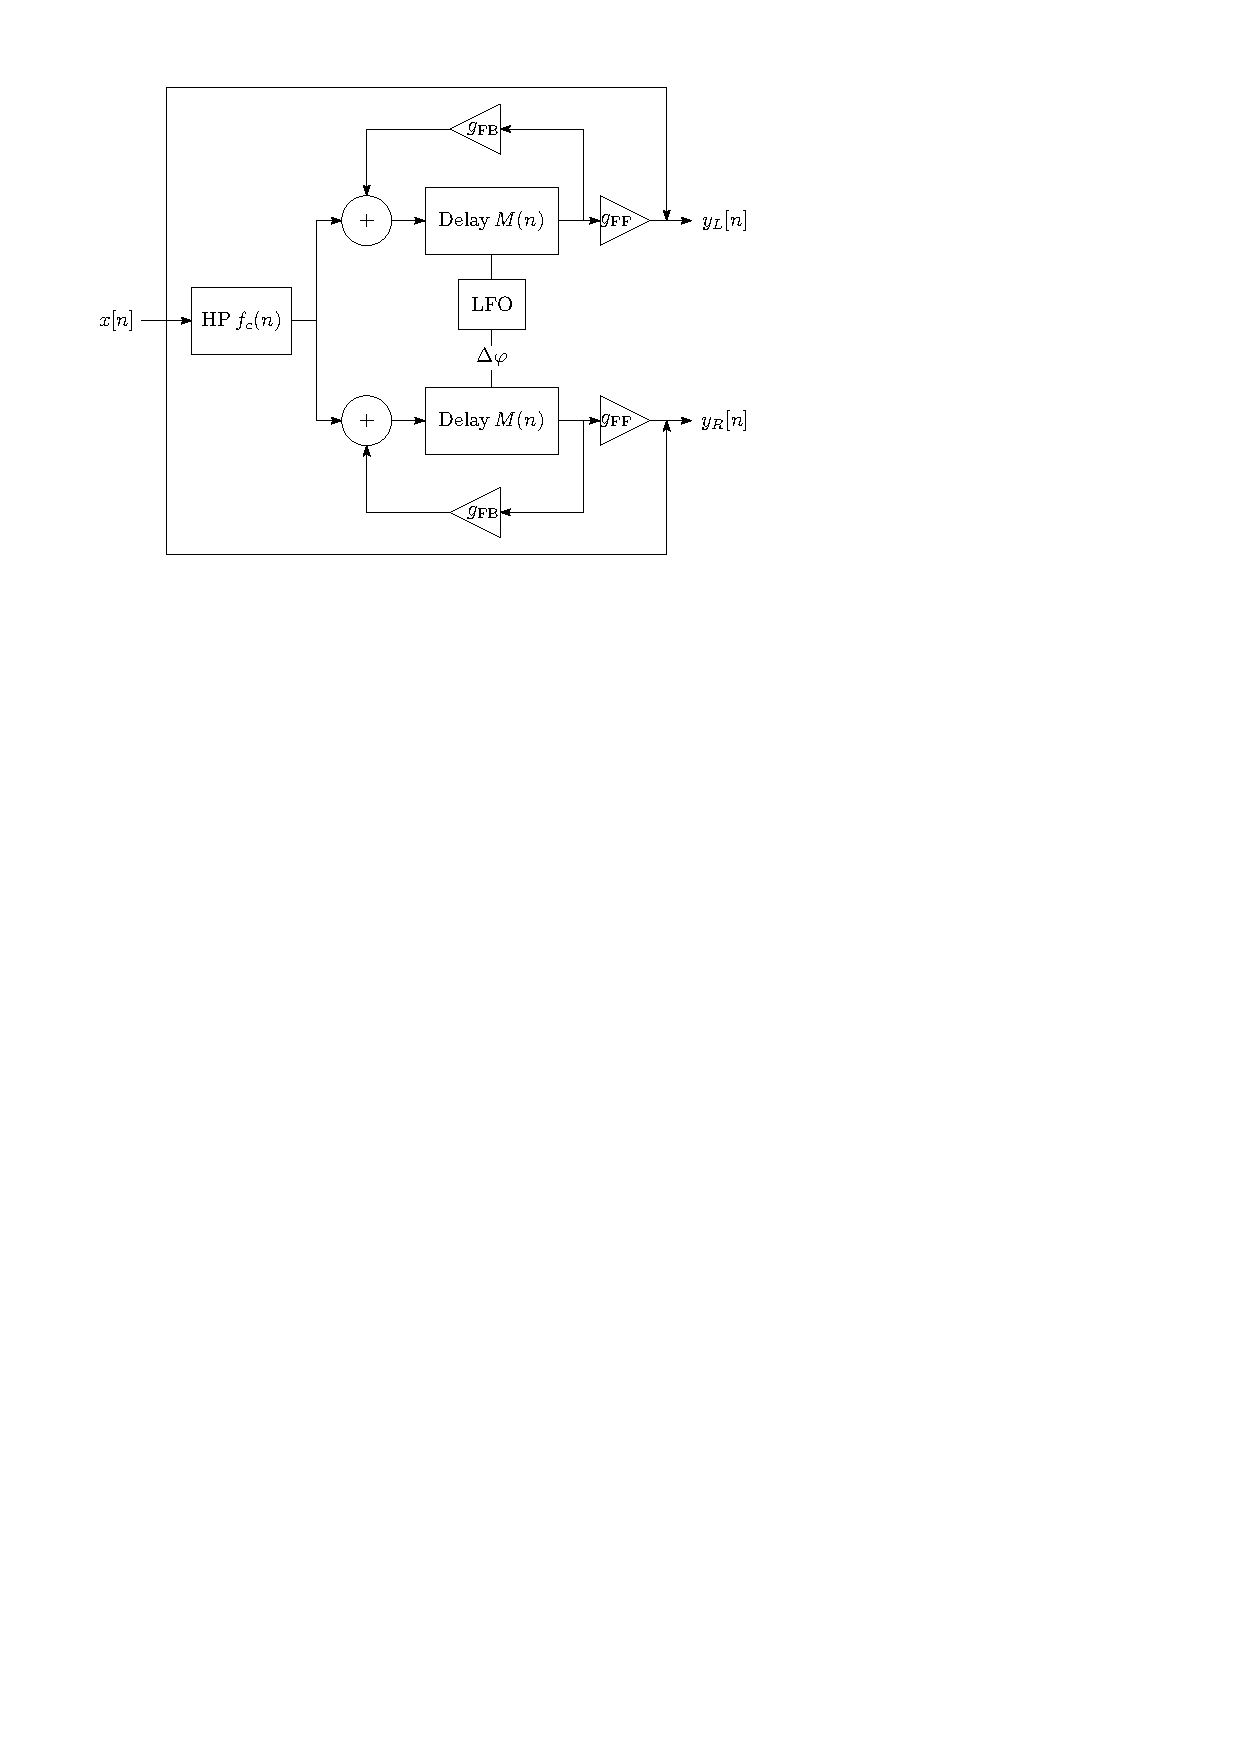
\includegraphics[width=0.6\linewidth]{assets/diagram-full.pdf}
	\caption{Complete full diagram}
	\label{fig:diag}
\end{figure}